\chapter{模型自动化划分方法设计与实现}
在上一章中,我们介绍了\sys{}的整体设计和各个模块的作用,分别介绍了能够将原始模型转化为计算图中间表示的模型结构分析模块(\ref{sec:convertion}),能够得到设备之间通信带宽模型的通信代价建模模块(\ref{sec:commu}),能够对计算图中每个节点显存用量进行估计的显存代价估计模块(\ref{sec:mem})以及能够得到计算图中每个节点的前向传播和反向传播的时间的计算代价分析模块(\ref{sec:time})。这四个模块旨在为最关键的模型划分模块提供必需的信息,用于进行模型划分。在进行模型划分时,从计算图的层面上,模型划分模块生成从节点到设备的映射,本章将重点介绍\sys{}中使用的模型自动化划分方法。

% 问题形式化定义
% 图优化算法
% 图划分算法
\section{模型划分的形式化定义}
\label{sec:formul}
% 1. 符号表示约定
首先我们对模型划分的问题进行形式化定义,模型的划分也就是计算图的划分。
计算图是有向无环图(Directed Acyclic Graph, DAG),在计算图中,每个节点都表示一个计算过程,每条边都表示一个依赖关系,边的终点依赖与边的起点,所以要求计算图中不能有环,也就是从一个节点出发的路径不能再回到该节点,无环的特性保证了不会出现环形依赖,确保计算过程可以正确进行。

一个计算图可以由$\mathcal{G}=\langle \mathcal{V}, \mathcal{E}, \mathcal{V}_{\mathit{in}}, \mathcal{V}_{\mathit{out}} \rangle $四元组表示,除了节点集$\mathcal{V}$ 和边集$\mathcal{E}$ 之外,还有用于表示计算图入口节点的$\mathcal{V}_\mathit{in}$ 和计算图出口节点的 $\mathcal{V}_{\mathit{out}}$。
$\mathcal{V}_{\mathit{in}}$是入度为0的节点的集合,对应到神经网络模型中,就是读入训练数据的节点。
$\mathcal{V}_{\mathit{out}}$ 是出度为0的节点的结合,对应到神经网络模型中就是输出预测结果的节点。
图 \ref{fig:graph-example} 展示了一个典型的计算图,其中$\mathcal{V}_\mathit{in}$和$\mathcal{V}_\mathit{out}$中的节点被标记为红色。

\begin{figure}[h]
	\centering
	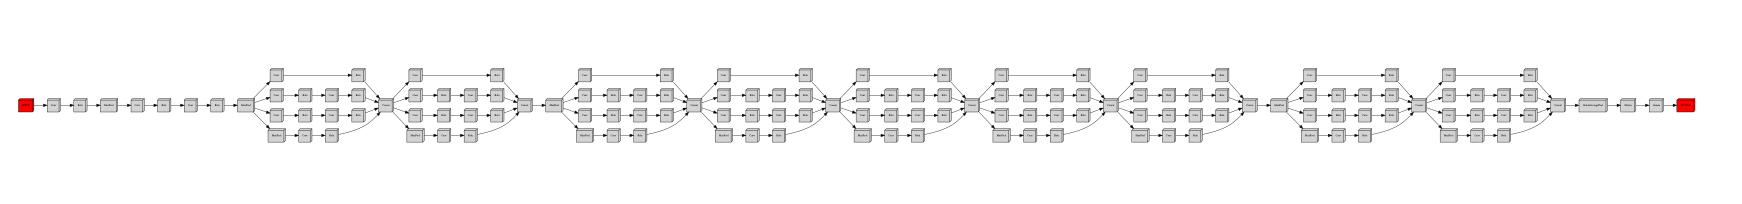
\includegraphics[width=\textwidth]{figure/4-alg/googlenet.png}
	\caption{GoogLeNet\upcite{googlenet} 的计算图}
	\label{fig:graph-example}
\end{figure}

\begin{table}[h]
	\centering
	\caption{模型划分模块的输入}
	\label{table:symbol}
    \begin{tabularx}{\linewidth}{p{3cm} p{3.2cm} X }
        \toprule
        \textbf{输出模块} & \textbf{符号表示} & \textbf{描述} \\
        \midrule
        \multirow{2}*{显存估计} & $\mathit{weight}_u$ & 节点$u$的参数所使用的显存,其中$u\in V$ \\
        \cmidrule{2-3}
        & $\mathit{size}_t$ & 中间变量$t$所使用的内存,通常来说,$t$对应$\mathcal{G}$中的某一条边,但是也有可能一个变量对应多个边,例如一个节点的输出变量可能是多个节点的输入边量。\\
        \midrule
        \multirow{2}*{计算代价分析} & $\mathit{FP}_{u}$ & 计算图中节点$u$的进行前向传播的计算用时,$u\in V$\\
        \cmidrule{2-3}
        & $\mathit{BP}_{u}$ &  计算图中节点$u$的进行反向传播的计算用时,$u\in V$\\
        \midrule
        通信建模 & $\mathit{Commu}(x,p,q)$ & 表示设备$p$和设备$q$之间传输数据量$x$的通信用时,如果$p=q$,则通信代价可以忽略不计。$Commu$就是设备之间的通信代价模型。 \\
        \bottomrule
    \end{tabularx}
\end{table}

$\mathcal{G}=\langle \mathcal{V}, \mathcal{E}, \mathcal{V}_{\mathit{in}}, \mathcal{V}_{\mathit{out}} \rangle $ 四元组由模型转换模块生成,并作为模型划分模块的一个输入,除了$\mathcal{G}$之外,模型划分模块还接受来自其他模块的输入,表 \ref{table:symbol} 中列举了除$\mathcal{G}$ 之外,模型划分模块接受的其他输入,以及这些输入的符号表示。
其中$\mathit{Commu}$是设备之间的通信代价模型。
对于每一对设备$p, q$,通信建模模块采集若干次设备之间点对点通信用时,通过线性拟合的方式构建设备之间的通信代价模型,模型接受通信数据量$x$,返回通信用时。

% 2. 问题的形式化定义
我们用$D$表示所有设备的集合,那么进行模型划分可以被看作寻找映射:$f: \mathcal{V}\mapsto D$,即为每个节点分配一个设备。
模型划分结果应该尽可能提升整个训练流程的数据吞吐量(Data Throughput)。
数据吞吐量表示了一个系统处理数据的速度,通常表示为单位时间内系统处理的数据量,当处理的数据量很大时,提高数据吞吐量就十分有必要。
在深度神经网络的训练中,数据吞吐量通常指单位时间训练完成的样本的数目,比如在视觉任务中,可以是每秒钟训练的图片数目,在自然语言处理任务中,可以是每秒钟训练的词向量数目。
提升数据吞吐量可以直接提升训练速度,缩短训练时间,因此模型划分模块以提升数据吞吐量为目标进行模型划分。
式 \ref{eq:target}描述了模型划分的目标,即在给定的硬件和计算图时,寻找可以使数据吞吐量(式中由$\mathcal{F}_{\mathit{throughput}}$表示)最大的划分,并满足显存约束。
\begin{equation}
	\label{eq:target}
	\begin{aligned}
		& \argmax_{f:\mathcal{V}\mapsto D} & \mathcal{F}_{\mathit{throughput}}(\mathcal{G}, D, f:\mathcal{V}\mapsto D) \\
		& \mathrm{s.t.} &\mathit{Memory}\ \mathit{Constraints}
	\end{aligned}
\end{equation}

\begin{equation}
	\label{eq:target2}
	\begin{aligned}
		& \argmin_{f:\mathcal{V}\mapsto D} & \mathcal{F}_{\mathit{iteration}}(\mathcal{G}, D, f:\mathcal{V}\mapsto D) \\
		& \mathrm{s.t.} &\mathit{Memory}\ \mathit{Constraints}
	\end{aligned}
\end{equation}

模型的训练具有迭代式的特性,每一轮迭代中模型对相同大小的数据批进行前向传播,通过损失函数计算损失,并且进行反向传播和参数优化。
每一轮迭代所需用时基本相同,因此最大化数据吞吐量等价于最小化单次迭代处理时间(Time Per Iteration )。
所以,式\ref{eq:target}也等价于式\ref{eq:target2},即寻找能最小换单次迭代用时的模型划分,其中单次迭代时间由$\mathcal{F}_{\mathit{iteration}}$表示。

\begin{figure}[h]
	\centering
	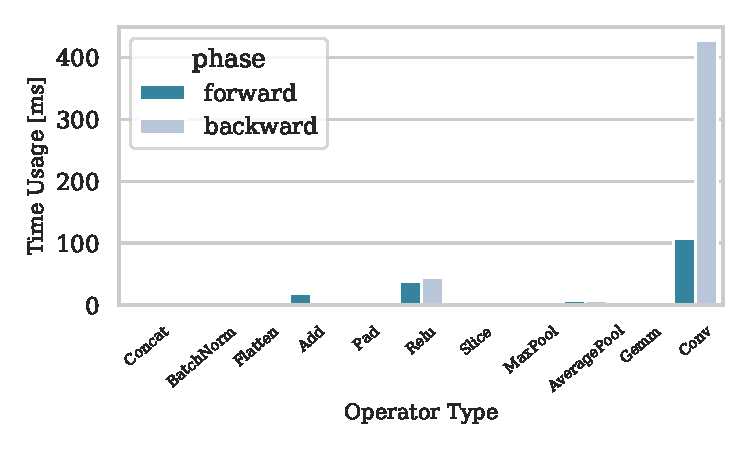
\includegraphics[width=0.85\textwidth]{./figure/4-alg/fp_bp.pdf}
	\caption{前向传播(FP)用时和反向传播(BP)用时的对比}
	\label{fig:fp-vs-bp}
\end{figure}

单次迭代时间是训练过程中,模型处理一个数据批的用时,包括前向传播和反向传播用时。
而现有的一些工作中,如Pesto \upcite{pesto} 中,简单的将单次迭代处理时间等价于计算图的执行用时,也就是训练过程中前向传播的用时,而忽略了反向传播的用时。
反向传播的代价不应该被忽略,图 \ref{fig:fp-vs-bp} 展示了在Amoebanet-D网络中,不同类型的算子的前向传播用时之和和反向传播用时之和。
可以发现,对于模型中的主要计算负载,二维卷积算子(Conv2D)的反向传播用时远远大于前向传播用时,因此在计算单次迭代用时时,算子反向传播的用时不能忽略。


\section{基于约束优化的模型划分}
\label{sec:algorithm}
% 简单介绍各个方向,然后说约束优化是主流
模型划分问题可以看作是带有通信依赖的任务调度问题在深度学习训练中的一种体现。
可以将计算图中的各个节点看作是一些有依赖关系的任务,将设备看作是一系列可以运行任务的处理器。
任务之间的依赖关系通过通信定义,如果任务B依赖任务A,则任务B需要通过通信获取任务A的输出,作为自己的输入。
被调度在相同处理器上的任务之间的通信时间可以忽略。
带有通信依赖的调度问题已经被证明是NP-Hard问题 \upcite{sched},因此无法在多项式时间内求出最优解。

现有工作 \upcite{rl1,rl2,baechi} 使用强化学习方法和近似算法进行模型划分,但是强化学习方法需要进行多次尝试和长时间的训练才能收敛。
而近似算法的使用场景较为有限,仅在通信计算比(Communication Computation Ratio, CCR)接近1时具有较好的近似比,而对于结构比较复杂的模型,由于计算图中边的数目较多,因此通信代价更大,CCR更大,所以近似算法难以获得较好的划分。
Hafeez等提出了Pesto\upcite{pesto},引入了约束优化方法进行模型划分。
本节接下来会首先会简单介绍Pesto中的约束优化算法以及其不足之处(\ref{sec:pesto}),然后详细介绍\sys{}中使用的约束优化算法(\ref{sec:core})和\sys{}中用来减少问题规模的节点协同放置算法(\ref{sec:co-place}),最后介绍\sys{}中的约束优化问题求解的实现(\ref{sec:picos-implement})。


\subsection{Pesto的约束优化}
\label{sec:pesto}
式\ref{eq:p-target} 到式\ref{eq:pst7} 给出了Pesto中对于模型划分约束优化的定义。
在Pesto中,假设原始的计算图表示为$\mathcal{G}=\left\langle \mathcal{E}, \mathcal{V}, \mathcal{V}_{in}, \mathcal{V}_{out}\right\rangle $。Pesto会预先对计算图进行修改,对于图中的每一个有向边$e=\left\langle i,j \right\rangle\in\mathcal{E}$,Pesto都会添加一个新的节点$k$,来表示节点$i$和节点$j$之间的通信,同时会用边$\left\langle i,k\right\rangle $和边$\left\langle k,j\right\rangle $替换边$\left\langle i,j\right\rangle $。
这样被修改后的图被表示为$\mathcal{G}=\left\langle \mathcal{\overline{E}},\mathcal{\overline{V}},\mathcal{\overline{V}}_{in},\mathcal{\overline{V}}_{out} \right\rangle$。
表示通信的节点的集合被记为$\mathcal{O}_{GG}$。


% Pesto的约束
\begin{align}
	& \mathrm{min} & &\mathcal{C}_{\mathit{max}} \label{eq:p-target}\\
	& \mathrm{s.t.} & &\mathcal{C}_i \le \mathcal{S}_j \quad \left\langle i,j \right\rangle\in \mathcal{\overline{E}}  \label{eq:pst1}\\
	& & &\mathcal{S}_i + p_i = \mathcal{C}_i  \quad\forall i\in \{\overline{\mathcal{V}} / \mathcal{O}_{GG} \}  \label{eq:pst2}\\
	& & &0\le \mathcal{C}_i\le \mathcal{C}_{\mathit{max}} \quad\forall i\in \overline{\mathcal{V}} \label{eq:pst3}\\
	& & & z_k = x_i \otimes x_j \quad\forall k \in \mathcal{O}_{GG}, (i,k),(k,j)\in\overline{\mathcal{E}} \label{eq:pst4}\\
	& & & S_i + z_i p_i = C_i \quad \forall i \in \mathcal{O}_{GG}\label{eq:pst5} \\
	& & & x_i \in \{0,1\} \quad\forall i \in \mathcal{O}_{GG} \label{eq:pst6}\\
	& & & \text{Memory Constraints and other constraints.} \label{eq:pst7}
\end{align}

在Pesto的约束优化问题的定义中,式\ref{eq:p-target}给出了约束优化要优化的目标,即最大完成时间。
约束\ref{eq:pst1} 表示对于计算图中的每条边$\left\langle i,j\right\rangle $,都有节点$j$的开始时间大于等于节点$i$的完成时间,即表达了各个节点之间的依赖关系。
约束\ref{eq:pst2} 表示对于每个非通信节点$i$,都有结束时间$\mathcal{C}_i$等于开始时间$\mathcal{S}_i$加上该节点的计算用时$p_i$。
约束\ref{eq:pst3} 定义了优化目标$\mathcal{C}_{max}$的下限,即整个计算图的执行时间应该在所有节点执行完成后。
约束\ref{eq:pst4} 定义一组指示随机变量(Indicator Variables) $z_k$,对于$\mathcal{O}_{GG}$中的节点$k$,如果它两端的节点$i$和$j$在同一个设备上,即$x_i=x_j$,则$z_k=0$,否则$z_k=1$。
对于通信节点$i$,约束\ref{eq:pst5}会根据$z_i$的值计算通信结束的时间,如果参与通信的两个节点在同一个设备上,则通信用时可以忽略,因此有$\mathcal{C}_i=\mathcal{S}_i$,否则需要考虑通信用时$p_i$。
Pesto的约束只适用于设备数目为2的场景,因此在约束\ref{eq:pst5}中,用于指示节点$i$最终被划分到哪个设备的变量$x_i$的取值是0或者1,但是在多个设备的情况下,需要进行扩展。
最后,Pesto加入了内存约束以及其他有关通信的约束。

尽管Pesto给出了用约束优化进行模型划分的思路,但是从Pesto给出的约束优化问题的定义来看,仍然有一些不足之处:
\begin{itemize}
	\item Pesto只考虑了设备数目为2的情况:在设备数目为2时,可以通过简单的异或运算确定两个节点是否在同一台设备上,但是需要扩展到多个设备的场景时,需要更复杂的约束条件。无法只通过一个二元变量来简单的表达节点被划分到哪个设备上。
	\item Pesto没有考虑通信的异构性:对于设备数目为2的情况,由于设备之间只有一条通信链路,因此可以简单的通过$p_i$来表示通信过程$i$的用时,但是在真实场景中,当设备数目大于2时,设备之间通常有多条通信链路,这些通信链路往往是异构的,通信过程$i$发生在不同的通信链路上可能对应不同的通信用时,Pesto的约束条件并没有加入对与通信异构性的考虑。
	\item Pesto没有考虑反向传播:在Pesto的约束中,最小化的目标是计算图的执行时间,也就是所有节点完成前向传播的时间。在训练过程中,单次迭代用时由前向传播和反向传播两部分的用时构成,而反向传播的用时无法忽略,因此只有在优化目标和约束中加入有关反向传播的部分才可以更准确的指导模型的划分。
	\item 缺少显存约束的详细表达:每个设备上的节点和变量使用的显存数目不能超过当前设备的最大容量,而Pesto没有给出显存约束的详细表达。
\end{itemize}

\subsection{\sys{}的约束优化}
\label{sec:core}
\begin{align}
	& \text{min} & & \mathit{Makespan} \label{eq:op-target} & \\
	& \text{s.t.} & & \mathcal{S}_{fp,i}=0 &\Gamma^{-}(i)=0, i\in \mathcal{V} \label{eq:cons1}\\
	& & & \mathcal{S}_{bp,i}=\mathcal{C}_{fp,i} &\Gamma^{+}(i)=0,i\in \mathcal{V}\nonumber \\
	& & & \mathcal{C}_{fp,i} = \mathcal{S}_{fp,i} + \mathit{FP}_i & \forall i\in \mathcal{V} \label{eq:cons2}\\
	& & & \mathcal{C}_{bp_i} = \mathcal{S}_{bp,i} + \mathit{BP}_i & \forall i\in \mathcal{V}\nonumber \\
	& & & \mathit{Makespan} \ge \mathcal{C}_{bp,i} & \forall i\in \mathcal{V} \label{eq:cons3} \\
	& & & \sum_{p=1}^{m} \mathcal{X}_{i,p}=1, \mathcal{X}_{i,p}\in\{0,1\} & \forall i\in \mathcal{V} \label{eq:cons4} \\
	& & & \mathit{Commu}_{i,j} = \sum_{p\neq q}\mathcal{X}_{i,p}\mathcal{X}_{j,q}F_{\mathit{commu}}(i,j,p,q) & \forall \left\langle i,j\right\rangle \in \mathcal{E} \label{eq:cons5}\\
	& & & \mathcal{S}_{fp,j} \ge \mathcal{C}_{fp,i} + \mathit{Commu}_{i,j}, \mathcal{S}_{bp,i} \ge \mathcal{C}_{bp,j} + \mathit{Commu}_{i,j} &\forall \left\langle i,j\right\rangle \in \mathcal{E} \nonumber \\
	& & & \text{Memory Constraint.} \label{eq:cons6}
\end{align}
	
式\ref{eq:op-target}~\ref{eq:cons6} 给出了\sys{}中对于模型划分的约束优化问题的定义。
表\ref{table:symbol2} 中给出了\sys{}的约束优化问题中用到的变量,以及对这些变量的解释。
% \begin{table}[h]
% 	\centering
% 	\caption{\sys{}约束求解问题中的变量符号表示}
% 	\label{table:symbol}
%     \begin{tabularx}{\linewidth}{p{3cm} p{3.2cm} X }
%         \toprule
%         \textbf{输出模块} & \textbf{符号表示} & \textbf{描述} \\
%         \midrule
%         \multirow{2}*{显存估计} & $\mathit{weight}_u$ & 节点$u$的参数所使用的显存,其中$u\in V$ \\
%         \cmidrule{2-3}
%         & $\mathit{size}_e$ & 边$e$的起始节点的输出变量的大小,该变量作为边$e$的终点的输入,其中$e\in E$ \\
%         \midrule
%         \multirow{2}*{计算代价分析} & $\mathit{FP}_{u}$ & 计算图中节点$u$的进行前向传播的计算用时,$u\in V$\\
%         \cmidrule{2-3}
%         & $\mathit{BP}_{u}$ &  计算图中节点$u$的进行反向传播的计算用时,$u\in V$\\
%         \midrule
%         通信建模 & $\mathit{Commu}(x,p_1,p_2)$ & 表示设备$p_1$和设备$p_2$之间传输数据量$x$的通信用时,如果$p_1=p_2$,则通信代价可以忽略不计。$Commu$就是设备之间的通信代价模型。 \\
%         \bottomrule
%     \end{tabularx}
% \end{table}

\begin{table}[h]
	\centering
	\caption{\sys{}约束求解问题中的变量符号表示}
	\label{table:symbol2}
    \begin{tabularx}{\linewidth}{p{2.8cm}  X }
        \toprule
        \textbf{符号名称} & \textbf{描述} \\
        \midrule
        $\mathcal{S}_{fp,i}$  &在一次完整的前向传播和反向传播中,节点$i$进行前向传播的开始时间。\\
        \midrule
        $\mathcal{S}_{bp,i}$ & 在一次完整的前向传播和反向传播中,节点$i$进行反向传播的开始时间。 \\
        \midrule
        $\mathcal{C}_{fp,i}$ &在一次完整的前向传播和反向传播中,节点$i$前向传播的结束时间。\\
        \midrule
        $\mathcal{C}_{bp,i}$ &在一次完整的前向传播和反向传播中,节点$i$反向传播的结束时间。\\
        \midrule
        $\mathit{FP}_i$ & 节点$i$进行前向传播的用时,该用时由\textbf{计算代价估计}模块给出。\\
        \midrule
        $\mathit{BP}_i$ & 节点$i$进行反向传播的用时,该用时由\textbf{计算代价估计}模块给出。\\
        \midrule
        $F_{\mathit{commu}}(i,j,p,q)$ & 假设节点$i$被划分到设备$p$上,节点$j$ 被划分到设备$q$上,则$i$和$j$通过设备$p$和设备$q$之间到通信链路进行通信的用时为$\mathit{F_{\mathit{commu}}}(i,j,p,q)$。因为节点$i$和节点$j$之间通信的数据量是已知的,因此该用时可以由\textbf{通信代价建模}模块给出的$\mathit{Commu}(x,p,q)$进一步计算得到。\\
        \midrule
        $\mathcal{X}_{i,p}$ & 用于表示划分结果的指示变量,也是待求解的变量。$\mathcal{X}_{i,p}=1$ 表示节点$i$ 被划分到了设备$p$上。\\
        \midrule
        $\mathit{Cap_p}$ & 设备$p$的显存容量。在进行训练前,可以通过使用NVML库 \cite{nvml}采集硬件信息得到。\\
        \midrule
        $\mathit{Makespan}$ & 优化目标,模型训练中单次迭代用时。 \\
        \bottomrule
    \end{tabularx}
\end{table}

% 我们的约束
为了得到更好的模型划分,\sys{}提出了新的约束优化的方法。
具体的,每个约束的含义如下:
\begin{itemize}
	\item 式\ref{eq:op-target} 定义了约束优化问题的优化目标,即最小化训练过程中单次迭代的用时。
	\item 式\ref{eq:cons1} 约束了计算图的入口节点,即入度($\Gamma^{-}(i)$)为0的节点的前向传播开始时间为0。
	因为对于计算图的入口节点来说,前向传播不依赖于任何其他节点,因此可以立刻开始。
	类似的,对于计算图的出口节点,即出度($\Gamma^{+}(i)$)为0的节点的反向传播的开始时间等于该节点的前向传播结束时间。
	\item 式\ref{eq:cons2}约束了节点的前向/反向传播结束时间等于开始时间加计算用时。
	\item \ref{eq:cons3} 约束了优化目标$\mathit{Makespan}$ 不小于所有节点的反向传播完成时间。
	\item 式\ref{eq:cons4} 定义了一组指示随机变量用来表示节点的划分情况,同时约束了每个节点恰好被划分到一个设备上。
	\item 式\ref{eq:cons5} 定义了通信代价,以及通信代价对总体用时的影响。对于$\mathcal{E}$中的每条边$\left\langle i,j\right\rangle $,$i$和$j$之间的通信代价$\mathit{Commu}_{i,j}$由节点$i$和节点$j$的划分情况决定。
\end{itemize}

对于显存约束\ref{eq:cons6},我们需要计算在某个划分下设备$p$上的显存占用量,占用量分成两部分来计算,一部分是在被划分到设备$p$上的节点的参数/梯度/动量等使用的显存,这部分只和节点有关。
另一部分是设备$p$上的变量的显存占用,一个变量可能与多个节点相关联,例如某个变量可以同时作为多个节点的输入,这里使用$R(j)$表示与变量$j$关联的节点的集合。
当与该变量相关联的任意节点被放置到设备$p$上,该变量就会占用设备$p$的一部分显存,因此最后得到的显存约束为式\ref{eq:mem-cons}。

\begin{equation}
	\label{eq:mem-cons}
	\mathit{Cap}_p \ge \alpha  \sum_{i\in V} \mathcal{X}_{i,p} \mathit{weight}_i + 2\cdot \sum_{j\in \mathcal{G}.\mathit{variables}} \mathit{max}(\{\mathcal{X}_{i,p} |  i\in R(j)\}) \mathit{size}_{j}
\end{equation}

在显存约束中,$\alpha$是和优化器有关的常量,如果优化器需要使用动量或者二阶动量来调整梯度下降的方向,那么我们需要参数大小常数倍的空间来存储这些额外的信息,例如使用Adam优化器 \upcite{adam}时,优化器需要使用梯度、动量以及二阶动量,因此此时的$\alpha$被设置为4。

在式\ref{eq:mem-cons}的第二部分,如果与变量$j$关联的节点中,存在被划分到设备$p$上的节点,那么就需要考虑变量$j$对设备$p$的显存占用的影响。如果$R(j)$中的所有节点都没有放置在设备$p$上,即$\mathit{max}(\{\mathcal{X}_{i,p} |  i\in R(j)\})=0$,那么变量$j$不会使用设备$p$上的显存,这部分用量也不会被考虑。

\sys{}的约束优化弥补了Pesto中的不足,将问题扩展到任意数目的设备,同时考虑了设备之间通信链路的异构性,对通信进行了更准确的建模。
并且\sys{}在优化目标和约束中加入了对反向传播的考虑,更加准确的建模了模型训练过程中的计算代价,同时也给出了对显存约束的准确描述。

\subsection{节点协同放置}
\label{sec:co-place}
% 为什么需要节点协同放置: 减小问题规模
% 节点协同放置的思路: 减小CCR
% 算法 + 如何整合
通常来说,一个大型神经网络模型的计算图中会有几千甚至上万个节点,在约束优化问题的定义式\ref{eq:target}中,约束的数目和节点的数目以及计算图中边的数目都呈现出线性相关性。
因此直接使用对大型神经网络模型进行约束优化,问题的规模会十分巨大,约束优化求解器在面对上万个约束时,将难以保证求解的速度和质量,因此,我们希望通过对计算图进行预处理,来缩小问题的规模。


\begin{figure}[h]
	\centering
	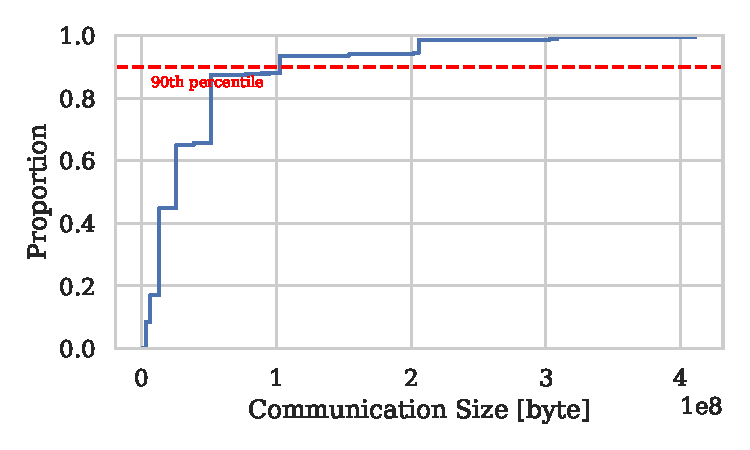
\includegraphics[width=0.85\textwidth]{./figure/4-alg/commmu_cdf.pdf}
	\caption{AmobaNet-D的计算图中通信代价的累积分布函数}
	\label{fig:commu-cdf}
\end{figure}

图\ref{fig:commu-cdf}展示了AmoebaNet-D模型的计算图中,所有边上的通信数据量的累积分布函数。
从图中可以发现,几乎$90\%$的通信数据量都低于$1\times 10^8$字节,大部分的通信都是较小的,只有少数的边具有较大的数据传输量,成为计算图中数据传输的瓶颈。
对于这类具有较大数据传输量的边,我们希望让边两端的节点被划分到相同设备上,从而避免边上较大的通信开销。

\sys{} 使用节点协同放置的方法,优先将通信开销较大的边两端的节点放置在同一个设备上。
一方面可以避免出现通信瓶颈,另一方面,可以有效减少约束优化中变量的个数。
\sys{}采用等价类(Equivalence Class)划分的思路对节点进行分组,
算法\ref{alg:co-place}描述了\sys{}进行节点协同放置的过程。

\begin{algorithm}[h]
	\caption{节点协同放置}
	\label{alg:co-place}
	\begin{algorithmic}[1]
	\REQUIRE 计算图:$\mathcal{G}$,设备列表:$\mathit{Devices}=\{p_1, p_2,\cdots, p_n\}$
	\ENSURE 节点到分组的映射: $\mathit{NodeToGroups}$
	\STATE $\mathit{NodeToGroups} \leftarrow \mathrm{Map}[\mathit{node}, \mathit{group}]$
	\STATE $\mathit{ds} \leftarrow \mathrm{NewDisjointSet}(\mathcal{G}.\mathcal{V})$
	\STATE $\mathit{totalMem}\leftarrow \sum_{i=1}^{n}p_i.\text{mem}$
	\STATE $\mathit{requireMem}\leftarrow \mathcal{G}.\text{mem}$
	\STATE $\mathit{maxGroupMem}\leftarrow \text{min}(\{p_1.\text{mem}, p_2.\text{mem}, \cdots, p_n.\text{mem}\})$
	\STATE $\mathit{minGroupNum}\leftarrow 2n$
	\IF{$\mathit{totalMem} < \mathit{requireMem}$}
		\STATE \textbf{RaiseError} "Insufficient Memory."
	\ENDIF
	\STATE $Q\leftarrow \text{SortByCommunicationSize}(\mathcal{G}.\mathcal{E})$ \quad\textcolor{gray}{\# 按照通信开销从大到小排序}
	\FOR{$\mathit{ds}.\mathit{size} \ge \mathit{minGroupNum}\quad \textbf{AND} \quad Q.\text{size} > 0$}
		\STATE $e\leftarrow Q.\text{pop()}$
		\IF{$\mathit{ds}.\text{Find}(e.u) = \mathit{ds}.\text{Find}(e.v)$}
			\STATE \textbf{continue}
		\ELSE
			\STATE $\mathit{newGroup} \leftarrow \mathit{ds}.\text{Find}(e.u) \cup \mathit{ds}.\text{Find}(e.v)$
			\IF{$\mathit{newGroup}.\text{mem} > \mathit{maxGroupMem}$}
				\STATE \textbf{continue} \quad \textcolor{gray}{\# 合并后NodeGroup过大,取消此次合并}
			\ELSE
				\STATE $\mathit{ds}.\text{Merge}(\mathit{ds}.\text{Find}(e.v, \mathit{ds}.\text{Find}(e.u)))$ \quad \textcolor{gray}{\# 进行合并}
			\ENDIF
		\ENDIF 
	\ENDFOR
	\FOR{$u\in \mathcal{G}.\mathcal{V}$}
		\STATE $\mathit{NodeToGroups}[u]\leftarrow \mathit{ds}.\text{Find}(u).\text{id}$
	\ENDFOR 
	\RETURN $\mathit{NodeToGroups}$
	\end{algorithmic}
\end{algorithm}


首先计算出计算图$\mathcal{G}$所需要的内存的总量和所有设备的可用内存,判断是否可以满足需求。
然后创建并查集(Disjoint Set),并查集是一种可以以接近常数时间复杂度的代价进行等价类的判断和合并的数据结构。
在初始化阶段,每个节点都位于不同的等价类中。
计算图中所有的边会按照通信代价从大到小进行排序,算法会优先检查通信代价较大的边,如果边两端的节点不属于同一个等价类,而且满足合并条件,则进行合并。
在合并过程中,节点组的数目不断减小,因此我们需要控制节点组的数目不会太小(小于设备数目),导致无法进行划分。
我们设置节点组的数目的下限为设备数目的2倍,当节点组数目低于下限时,停止合并。

当节点协同放置完成后,节点被分成了若干组。
同一组中的节点会被放置在同一个设备上,因此只需要简单修改约束优化问题\ref{eq:target},让同一组中的节点共享指示随机变量即可。
通过节点协同放置,\sys{}在进行约束优化的求解之前,将节点提前划分成了若干组,组内的节点共享指示随机变量,减少了带求解的变量的个数,可以有效减少求解的用时,并且提高求解的质量。

\subsection{实现:使用PICOS和Gurobi}
\label{sec:picos-implement}
本小节将介绍如何使用PICOS和Gurobi实现\ref{sec:core}中描述的约束优化问题的求解。

Gurobi \upcite{gurobi}是一款商业化的高性能线性规划(Linear Programming),整数规划(Integer Programming)和混合整数规划(Mixed Integer Programming)求解器。
Gurobi也可以用于二次规划(Quadratic Programming),具有高效、准确和灵活的特点,被广泛应用于各种优化问题的求解。
Gurobi采用了一系列优化技术和算法,如高效的分支界定算法、内点算法、割平面算法等,可以快速准确地求解各类优化问题。
作为商用求解器,Gurobi也提供了免费的学术许可证。
\sys{}使用Gurobi作为求解器,对\ref{sec:core}中描述的约束优化问题进行求解。

为了简化对Gurobi的使用,\sys{}使用PICOS \upcite{PICOS}作为Gurobi的前端。
PICOS的全称是“Python Interface for Conic Optimization Solvers”,它是Python的约束优化建模工具,它允许用户使用Python来对约束优化问题进行建模。
PICOS提供了方便的Python接口,用于构建和解决凸优化问题,它提供了符号表达式,约束组合等高级抽象方式来描述优化问题,在一定程度上可以简化约束优化问题的定义。
PICOS具有强大的可扩展性,支持包括Gurobi,MOSEK \upcite{mosek}等多种求解器作为约束优化问题求解的后端,PICOS可以自动将用户通过Python定义的约束优化问题转化为各个求解器的输入形式,并且调用求解器进行求解。

\begin{lstlisting}[language=Python, caption={约束优化求解的Python实现}]
import picos as pc
...
# 创建问题和优化目标
P = pc.Problem(name='NetSplit MQP Problem')
Makespan = pc.RealVariable(name='makespan', lower=0)
P.minimize = Makespan
# 为每个节点组创建指示随机变量
X = [[None,]*num_devices for _ in range(num_groups)]
for i in range(num_groups):
	for p in range(num_devices):
		X[i][p] = pc.IntegerVariable(lower=0,upper=1)
# 为每个节点声明变量S_fp, S_bp, C_fp, C_bp
S_fp, S_bp, C_fp, C_bp = [], [], [], []
for i in range(num_nodes):
	S_fp.append(pc.RealVaribel(lower=0.0))
	S_bp.append(pc.RealVaribel(lower=0.0))
	C_fp.append(pc.RealVaribel(lower=0.0))
	C_bp.append(pc.RealVaribel(lower=0.0))
...

# 约束1: 图的入口节点的前向传播开始时间为0
for i in entry_nodes:
	P.add_constraint(S_fp[i] == 0.0)
# 约束2: 图的出口节点反向传播开始时间等于前向传播结束时间
for i in exit_nodes:
	P.add_constraint(S_bp[i] == C_fp[i])
# 约束3: 每个节点的计算代价
for i in range(num_nodes):
	P.add_constraint(C_fp[i] == S_fp[i] + FP[i])
	P.add_constraint(C_bp[i] == S_bp[i] + BP[i])
# 约束4: Makespan大于所有节点完成反向传播
for i in range(num_nodes):
	P.add_constraint(Makespan >= C_bp[i])
# 约束5: 具有依赖关系的节点需要进行等待
for (i,j) in g.edges:
    P += S_fp[j] >= C_fp[i] + Commu[i][j]
    P += S_bp[i] >= C_bp[j] + Commu[i][j]
# 约束6: 每个Group只能被放在1个设备上
for group_idx in groups:
    P += pc.sum(X[group_idx]) == 1

P += Commu[u][v] >= pc.sum(comm_ij) 
... 
# 求解
P.solve(solver="gurobi")
# 获取结果
for i in range(num_groups):
	for p in range(num_devices):
		if X[i][p] == 1.0:
			group_to_device[i] = p
...
\end{lstlisting}

上面的代码展示了使用PICOS定义约束优化问题\ref{eq:target}的部分过程。
首先我们在代码中引入PICOS包,然后创建优化问题的实例\texttt{pc.Problem}。
然后我们定义一系列变量和优化问题的优化目标。
变量是表示优化问题中未知量的对象,在创建变量后可以进一步向问题中添加约束来描述变量应该满足的条件,在PICOS中,\texttt{RealVariable}和\texttt{IntegerVariable}是最常用的两种变量,分别用来表示连续的实数变量和整数型变量。
例如我们将指示每一个节点组放置的变量X定义为整数型变量,且它的值只能取到0或1,然后我们通过约束6来约束一个节点组要被放置且只能被放置在一个设备上。
在问题定义完成之后,调用\texttt{solve}方法,选择求解器,进行求解。

在\sys{}的约束优化问题\ref{eq:op-target}中,限制解的存在性的约束只有式\ref{eq:cons6},也就是显存约束。
当模型训练的显存用量超过设备可以提供的显存用量时,该优化问题无解。
当存在任意一种模型划分和放置方案可以满足显存约束时,则求解器一定可以寻找到该问题的一个解,在实际应用中,由于问题定义和数值精度等原因,该解不一定是最优解。
为了验证这种基于约束求解的模型划分方法的有效性,我们在后续章节(\ref{sec:evaluation})中对\sys{}得到的模型划分效果进行了评估。

\section{本章小结}
本章主要介绍了模型划分的问题的形式化定义以及基于约束优化的模型划分方法。
首先,我们在\ref{sec:formul} 中对问题进行了形式化的定义,模型的划分等同于计算图的划分,也就是寻找计算图中节点到设备的映射,以最大化模型训练时的数据吞吐量。
我们介绍了模型划分的输入以及对应的符号表示,并且论述了反向传播的用时对于模型划分的影响。
然后我们介绍了基于约束优化的模型划分方法,介绍了Pesto的约束优化问题的定义,并分析了Pesto的一些不足,例如未考虑反向传播用时对划分的影响,没有扩展到任意数目设备,没有考虑集群中通信链路的异构性等。
接着我们着重介绍了\sys{}的约束优化问题的定义和求解的实现。我们基于PICOS和Gurobi在Python中实现了问题的定义和求解。同时我们也介绍了用于优化通信的节点协同放置方法。

在后续章节(\ref{sec:evaluation})中,我们将介绍对\sys{}的实验评估。
